\newpage
\section{Podręcznik użytkownika}  %6
%Opis jak używać programu. Mogą być z zrzut ekranu razem z opisem. 
\subsection{Menu główne}
Menu główne w aplikacji "Operacja Kooperacja" zawiera pierwszą zagadkę w grze. Jest nią duży czerowny przycisk z napisem "CLICK HERE". Po wciśnięciu tego przycisku aplikacja zamyka się natomiast przyciisk z "żarówką" pozwala nam przejść dalej.
	\begin{figure}[!htb]
	\begin{center}
		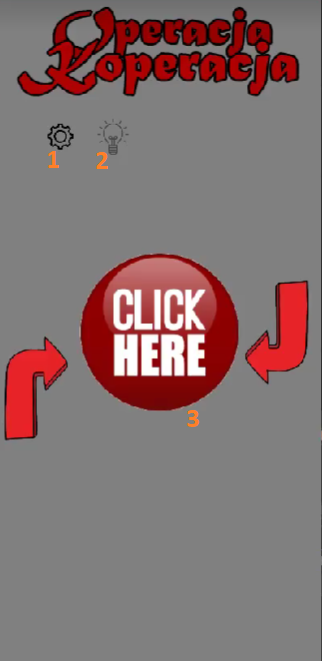
\includegraphics[width=8cm]{rys/opis1.png}
		\caption{Menu Główne}
		\label{rys:rysunek001}
	\end{center}
\end{figure}

\begin{enumerate}
	\item Przycisk pozwalający nam przejść do ustawień 
	\item Przycisk pozwalający nam przejść do właściwego menu głównego
	\item Przycisk ten wyłącza aplikacje 
\end{enumerate}

	\begin{figure}[!htb]
	\begin{center}
		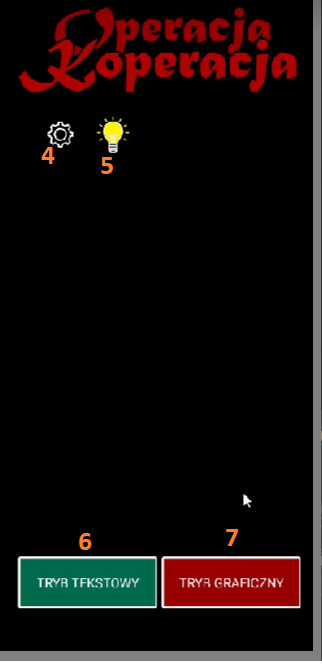
\includegraphics[width=8cm]{rys/opis3.png}
		\caption{Menu Główne v2}
		\label{rys:rysunek001}
	\end{center}
\end{figure}


\begin{enumerate}
	\setcounter{enumi}{3}
	\item Przycisk pozwalający nam przejść do ustawień 
	\item Przycisk pozwalający nam przejść do poprzedniego menu głównego
	\item Przycisk ten pozwala nam wybrać tryb tekstowy jako nasz tryb gry
	\item Przycisk ten pozwala nam wybrać tryb graficzny jako nasz tryb gry
\end{enumerate}

\subsection{Labirynt}
Po wybraniu graficznego trybu gry zostajemy przeniesieni do pierwszej zagadki, którą jest labirynt. Na początku dostajemy informacje o zagadce jak i kod do trybu tekstowego dla naszego partnera. Ta zagadka polega na doprowadzeniu postaci (pomarańczowego kwadratu) do wyjścia. Osoba w trybie graficznym widzi kilka wersji labiryntu i musi wybrać właściwy na podstawie informacji jakie dostanie od partnera, po czym musi poprowadzić osobę z trybu graficznego do wyjścia. Każde wejście w ściane kończy się utratą życia i zresetowaniem pozycji postaci.
	\begin{figure}[!htb]
	\begin{center}
		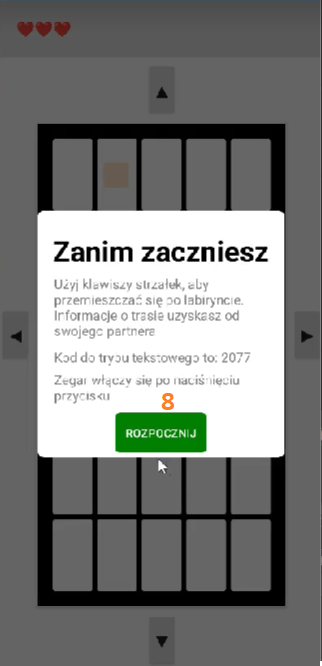
\includegraphics[width=8cm]{rys/opis2.png}
		\caption{Komunikat (Labirynt)}
		\label{rys:rysunek001}
	\end{center}
\end{figure}

\begin{enumerate}
	\setcounter{enumi}{7}
	\item Przycisk pozwalający nam rozpocząć grę
\end{enumerate}

	\begin{figure}[!htb]
	\begin{center}
		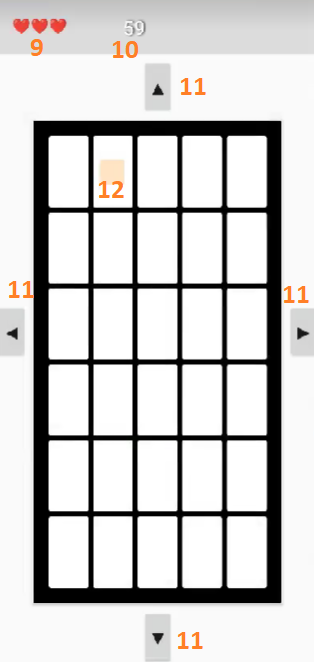
\includegraphics[width=8cm]{rys/opis4.png}
		\caption{Labirynt}
		\label{rys:rysunek001}
	\end{center}
\end{figure}

\begin{enumerate}
	\setcounter{enumi}{8}
	\item Licznik żyć (Zaczynamy mając 3 życia, w momencie utraty ostatniego przegrywamy)
	\item Timer (Pokazuje ile czasu mamy na daną zagadkę)
	\item Przyciski pozwalające poruszać naszą "postacią"
	\item Postać, którą sterujemy
\end{enumerate}